% !TeX root=main.tex
\chapter{「さわれる」遠隔学習システムの概要}
%%%%%%%%%%%%%%%%%%%%%%%%%%%%%%%%%%%%%%%%%%%%%%%%%%%%%%%%%%%%%%%%%%%%%%%%%%%%%%
\section{システムの目的}

2019年末に発生した新型コロナウイルス感染症 (COVID-19) の拡大により,人同士の
接触を避ける観点から,本邦でもほとんどの大学で講義・実験の遠隔化,オンライン化
を迫られました.特に実験・実習科目においては,いかに実地での実験・実習と同等の
教育効果を遠隔環境で達成するかが,重要な課題となります.また,もしもそのような
システムがあれば,たとえ実地での実験・実習が可能である場合でも,実験時間外の
自主学習に活用できます.

しかしながら,ディジタル回路や FPGA の学習におけるこれまでの遠隔学習システム
には,その操作から実際にハードウェアに触れているとの実感を得ることが難しい,
という問題点がありました.例えば,ACRi ルーム \cite{ACRi_Room}上の仮想マシン
には FPGA ボードが接続されているものの,そのスイッチや LED 等を直接操作・確認
することはできませんでした.

我々(愛知工業大学 工学部電気学科 ディジタルシステム研究室)がこの問題点に対する
解決法として開発したのが,本マニュアルで説明する,ディジタル回路の「さわれる」
遠隔学習システムです.以下,本マニュアルではこのシステムを SawareruSys と表記
します.詳しい学術的背景や,システムの設計・評価については,文献
\cite{TALE-fujieda} を参照してください.

%%%%%%%%%%%%%%%%%%%%%%%%%%%%%%%%%%%%%%%
\section{必要な機材・ソフトウェア一式}

遠隔実験の実施には,FPGAボードの入出力の変化を手元で確認するためのコントローラ
ボードが必要です.2024年3月現在,コントローラボードには以下の3つのバリエーション
があります.

\begin{enumerate}
 \item FPGA リモコンボード V2
 \item FPGA リモコンボード V4
 \item SawareruBoard V1
\end{enumerate}

\begin{figure}[ht]
 \centering
 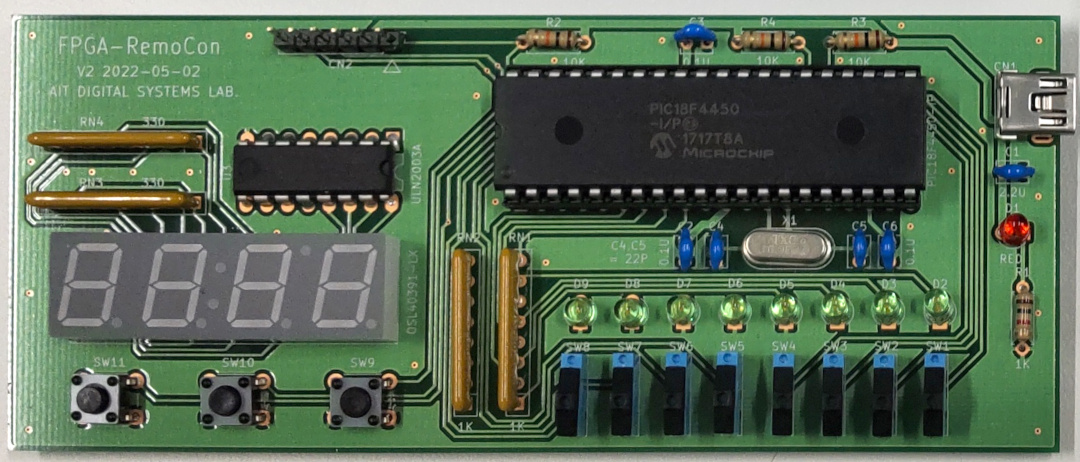
\includegraphics[width=80truemm]{figs/remocon_v2.jpg}
 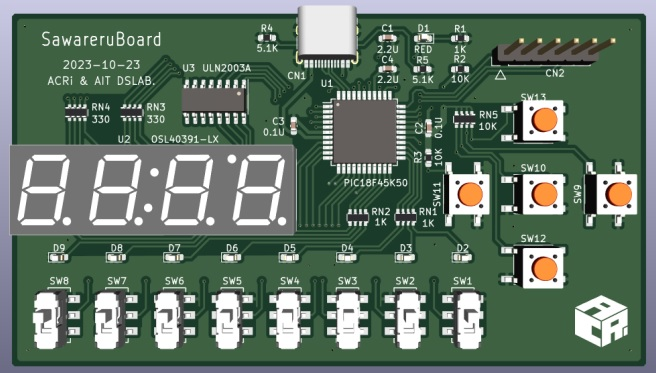
\includegraphics[width=60truemm]{figs/sawareru_v4.jpg}
 \caption{コントローラボードの例(左: FPGA リモコンボード V2,右: SawareruBoard V1).}
 \label{fig:boards}
\end{figure}

このうち1と3のボードの外景を,図\ref{fig:boards}に示します.
1のボードは,左・中央・右の3つのタクトスイッチを備え,PC との接続端子は USB
mini-B です.2と3のボードは機能的・形状的に同一で,十字型の5つのタクトスイッチ
を備え,接続端子は USB Type-C です.

また,SawareruSys の配布パッケージには,以下のファイル一式が含まれています.
\begin{itemize}
 \item DRFront: SawareruSys での開発を支援するためのフロントエンドツール
 \item Connectorアプリ: コントローラボードを遠隔サーバに接続するときに使用
 \item WinSCP: 遠隔サーバへファイルを転送するときに使用
\end{itemize}
加えて,Windows標準の以下のアプリケーションも使用します.
\begin{itemize}
 \item Windows PowerShell
 \item リモートデスクトップ接続
\end{itemize}

なお,WinSCP は Martin Prikryl 氏による著作物であり,GPL (version 3) ライセンス
に従って,ポータブル版の実行ファイルを再配布しています.ライセンスに関する詳細は,
配布パッケージの COPYING ファイルを参照してください.

%%%%%%%%%%%%%%%%%%%%%%%%%%%%%%%%%%%%%%%
\section{遠隔サーバの構成}

\begin{figure}[ht]
 \centering
 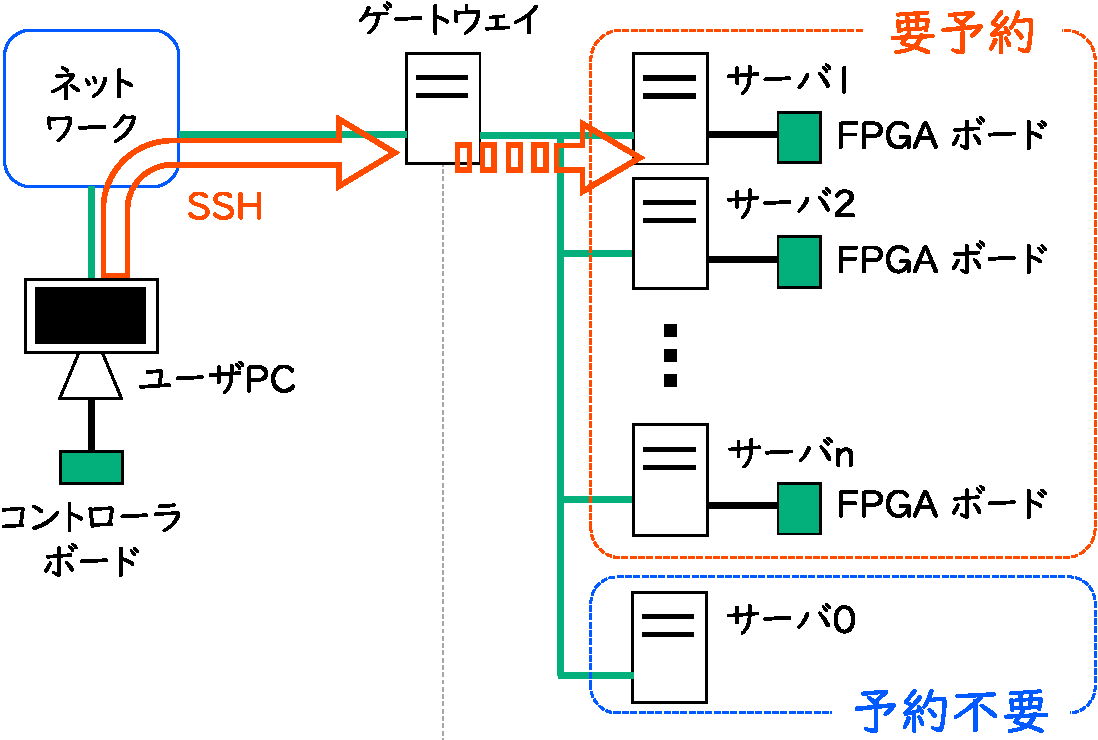
\includegraphics[width=80truemm]{figs/servers.pdf}
 \caption{遠隔サーバの構成図.}
 \label{fig:servers}
\end{figure}

SawareruSysにおける遠隔サーバの構成図を,図\ref{fig:servers}に示します.
遠隔サーバへの入口としてゲートウェイサーバが設置されており,ユーザは SSH 接続で
ゲートウェイサーバに接続します.開発用のサーバへのアクセスは,SSH ポートフォワー
ディング機能により間接的に行います.開発用のサーバには,FPGA ボードが1台ずつ設置
された予約の必要なサーバと,FPGA ボードが接続されていない予約不要のサーバとが
あります.

2024年3月時点の ACRi ルームでは,ゲートウェイサーバには fserv4,開発用のサーバには
vs000~vs910 の名前がつけられています.このうち末尾2桁が 00 であるサーバは予約不要
のサーバです.
愛工大の学内環境では,ゲートウェイサーバには gs1,開発用のサーバには ns0~ns5 の
名前がつけられています.ns0 は予約不要です.
予約が必要なサーバは,Web ブラウザで予約を行います.予約について詳しくは,各環境
のドキュメントまたは利用説明ページを確認してください.

PC と開発用のサーバでは,それぞれ別々の Connector アプリを起動して,通信の中継を
行います.PC とコントローラボード,サーバと FPGA ボードの通信には,それぞれで
USB-UART(USB を介したシリアル通信)を使用します.一方,PC とサーバとの通信は,
SSH ポートフォワーディングを介した TCP/IP 通信によります.このプロトコルの違いを
吸収し,通信の中継を行うのが,Connector アプリです.

%%%%%%%%%%%%%%%%%%%%%%%%%%%%%%%%%%%%%%%
\section{FPGA 内の回路構成}

SawareruSys では,入出力の遠隔操作を実現するために,FPGA 内部にあらかじめ入出力
制御回路を作りこんでおきます.ユーザは,入出力制御回路と接続されるユーザ回路部分
のみを開発します.

\begin{figure}[ht]
 \centering
 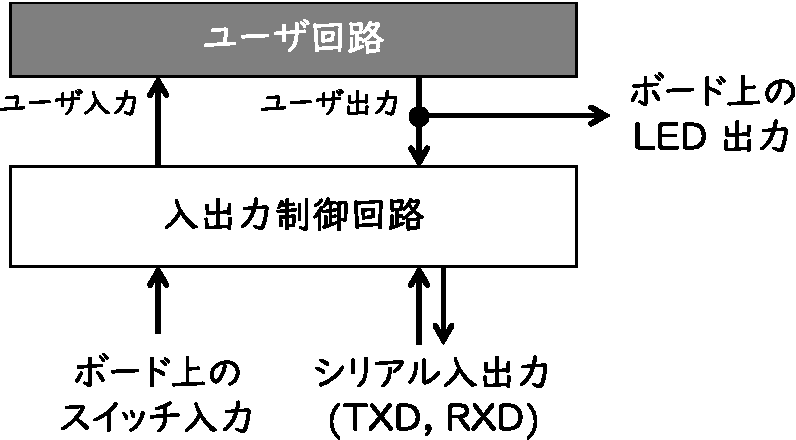
\includegraphics[width=80truemm]{figs/iocircuit.pdf}
 \caption{FPGA の内部構造の概要.}
 \label{fig:iocircuit}
\end{figure}

入出力制御回路とユーザ回路の関係の概要を,図\ref{fig:iocircuit}に示します.
入出力制御回路はシリアル通信の入出力(TXD と RXD)をもっており,サーバの
Connector アプリと接続されたかどうかや,入出力の変化の状況をチェックしています.
FPGAボードのスイッチ入力は,まず入出力制御回路に入ります.
サーバと接続されていない場合は,単にスイッチ入力の情報がユーザ回路の入力と
して渡されます.サーバと1度でも接続された場合は,入出力制御回路はコントローラ
ボードのスイッチの状態を受け取って保持し,その結果をユーザ回路の入力とします.
ユーザ回路の出力は,ボードの LED(または7セグメント LED)出力として使われる
ほか,入出力制御回路にも渡されます.
サーバと接続されている間,入出力制御回路はユーザ回路の出力の変化を監視し,
その結果をサーバに送ります.

SawareruSys では,ユーザ回路の入出力として,以下のものをサポートしています.
\begin{itemize}
 \item CLK: 100 MHz クロック 
 \item RST: リセットスイッチ(正論理)1 個
 \item SW(15)~SW(0): スライドスイッチ 16 個
 \item BTN{U, L, C, R, D}: タクトスイッチ 5 個(それぞれ,上,左,中央,右,下)
 \item LD(15)~LD(0): LED 16 個
 \item AN(7)~AN(0), CA~CG,DP: 7セグメント LED(負論理,8桁のダイナミック点灯)1 個
\end{itemize}
ただし,SW(15)~SW(8) はコントローラボードから操作できず,LD(15)~LD(8) と
7セグメント LED の左側4桁(AN(7)~AN(4) に対応)はコントローラボードから確認
できません.リセットスイッチは,ユーザ回路と入出力制御回路の両方をリセットします.
サーバと接続されていた場合には,接続されていない状態に戻りますので,ボードの
スイッチ入力が再び使えるようになります.

FPGA において,あらかじめ作りこまれた回路に自由に書き換えられるユーザ回路を
組み込んで使うための1つの方法に,動的部分再構成(DPR; Dynamic Partial
Reconfiguration)があります.AMD 社の FPGA における DPR 機能は,DFX(Dynamic
Function eXchange)とよばれます.DFX 機能を使うためには,同社の FPGA 開発環境
である Vivado 上で,多数のステップからなるスクリプトを実行する必要があります.
DRFront は,SawareruSys での DFX に必要な手順を自動化・効率化するために開発
されたフロントエンドツールです.

%%%%%%%%%%%%%%%%%%%%%%%%%%%%%%%%%%%%%%%
\section{サポートする FPGA ボード}

2024年3月現在,SawareruSys では Digilent 社の Nexys A7-100T,Arty A7-35T,
CMod A7-35T の3種類の FPGA ボードをサポートしています.

\subsection{Nexys A7-100T}

\begin{figure}[ht]
 \centering
 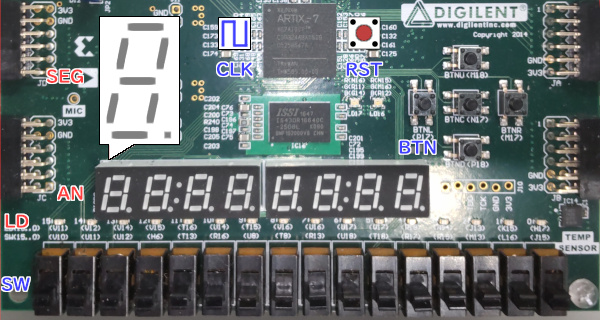
\includegraphics[width=90truemm]{figs/Nexys.jpg}
 \caption{Nexys A7-100T で使用できる入出力.}
 \label{fig:Nexys}
\end{figure}

Nexys A7-100T で物理的にアクセスできる入出力には,図\ref{fig:Nexys}に示す16個の
スライドスイッチ,5個のタクトスイッチ,16個のLED,8桁の7セグメント LED が含まれ
ます.これらすべてをユーザ回路上で扱えますが,スライドスイッチ・LED・7セグメント
LED のうち,左半分はコントローラボードでの確認・操作に対応していないことに注意
してください.リセットスイッチは,ボード右半分に2つ並んだ赤色のタクトスイッチ
のうち,左側のCPU RESET と書かれたスイッチです.

\subsection{Arty A7-35T}

\begin{figure}[ht]
 \centering
 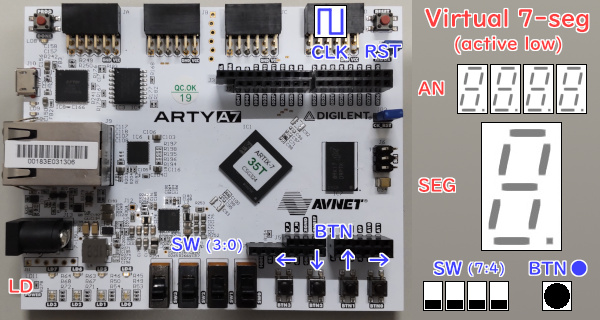
\includegraphics[width=90truemm]{figs/Arty.jpg}
 \caption{Arty A7-35T で使用できる入出力および仮想入出力.}
 \label{fig:Arty}
\end{figure}

Arty A7-35T は,Nexys A7-100T よりは安価なボードで,図\ref{fig:Arty}に示す
4個のスライドスイッチ,4個のタクトスイッチ(上下左右),8個のLEDに物理的に
アクセスできます.
LEDのうち4個は RGB LED ですが,SawareruSys では緑色の表示にのみ対応します.
コントローラボードを使って遠隔接続すると,仮想的に4桁の7セグメント LED と,
追加の4個のスライドスイッチ,1個のタクトスイッチ(中央)が利用できます.
リセットスイッチは,ボード右上の RESET と書かれたスイッチです.

\subsection{CMod A7-35T}

\begin{figure}[ht]
 \centering
 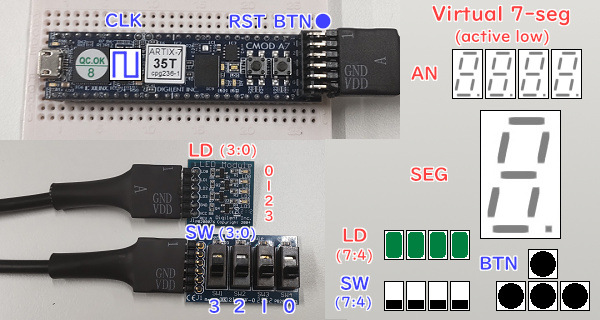
\includegraphics[width=90truemm]{figs/CMod.jpg}
 \caption{CMod A7-35T で使用できる入出力および仮想入出力.}
 \label{fig:CMod}
\end{figure}

CMod A7-35T は,ブレッドボードに差し込んで利用できる FPGA ボードで,サポートされて
いるボードの中では最も安価なボードですが,最小限の入出力装置しか備えていません.
そのため,Pmodケーブルキットの12ピン-デュアル6ピンケーブルを使用し,PMod 端子の
うち1~6ピンに PMod LED を,7~12ピンに PMod SWT を,それぞれ接続する使い方を
仮定します.接続例を図\ref{fig:CMod}に示します.あるいは,PMod 端子を使わずに,
ほぼすべてをコントローラボードから操作・確認する仮想入出力とみなすのもよいでしょう.

PMod 端子を使用した場合,CMod A7-35T を含む機材一式には,4個のスライドスイッチ,
1個のタクトスイッチ(中央),4個のLEDが含まれます.ボード上の2個のタクトスイッチ
のうち,ユーザ回路に接続されるのは右側のスイッチです.左側はリセットスイッチとして
使用します.コントローラボードを使って遠隔接続すると,4桁の7セグメント LED と,
追加の4個のスライドスイッチ,4個のタクトスイッチ(上下左右),4個の LED が仮想的
に利用できます.

PMod 端子を使用しない場合,CMod A7-35T には,1個のタクトスイッチ(中央)と3個の
LED が含まれます.ボード上の2個のタクトスイッチは,右側がユーザ回路に接続され,
左側がリセットスイッチとして使われます.
LEDのうち1個は RGB LED ですが,SawareruSys では緑色の表示にのみ対応します.
コントローラボードを使うと,4桁の7セグメント LED ,8個のスライドスイッチ,
追加の4個のタクトスイッチ(上下左右),5個の LED が仮想的に利用できます.

CMod A7-35T のボードに搭載されたオシレータの出力周波数は 12 MHz ですが,
SawareruSys ではこれをクロック生成回路(MMCM)で 100 MHz にしてから,ユーザ回路
および入出力制御回路に与えています.

%%%%%%%%%%%%%%%%%%%%%%%%%%%%%%%%%%%%%%%